%---------------------------------------------------------------------
%
%                          Cap�tulo 6
%
%---------------------------------------------------------------------

\chapter{Testings and Results}

\begin{FraseCelebre}
\begin{Frase}
At last the long wait is over \\
The weight is off my shoulders \\
I'm taking all control, yeah
\end{Frase}
\begin{Fuente}
Thomas \& Guy-Manuel, Daft Punk
\end{Fuente}
\end{FraseCelebre}

\begin{resumen}
Some tests were applied to main platform modules for the purpose of proving their proper functionality. Main capabilities that make the valuable the platform such as power consumption or spectrum sensing features have been tested. Descriptions of the carried out tests and corresponding results are exposed in this Chapter.  
\end{resumen}

%-------------------------------------------------------------------
\section{Test Model}
%-------------------------------------------------------------------
\label{cap6:sec:testModel}
%-------------------------------------------------------------------
The purposes of testing functionalities of the platform are to prove valuable capabilities and proper functionality of modules. Characterization is not expressely required and modules must respond to operation parameters provided by manufacturers. The already described  used firmware includes several test-benches to apply. Most of the software tools employed to test the platform are extracted, at least partially, from them. For a further description on the provided tests design, cosult \ref{juanpfc}. 

Tests are simple and check bounded functions. Aspects to check are related to sleeping modes operation and current consumption, microcontroller computing capabilities, spectrum sensing features and radio interfaces, or battery charger behaviour.   

%-------------------------------------------------------------------
\section{Energy management test}
%-------------------------------------------------------------------
\label{cap6:sec:consumptionTest}
%-------------------------------------------------------------------
This test tries to bring the \ac{CNGD} under different operation modes. On the one hand, different sleeping modes and energy options for \ac{RI}s and \ac{MCU} are achieved consecutively. On the other hand, consumed current by the platform is measured at each situation. 
This test was already included at the firmware and just few changes were needed to fully carry it out. These changes suppose the functions to control the power at the \ac{RI}s and they are described at Section \ref{cap7:subsec:usbtraces}.  

8 Different situations are configured. Following description covers the initial state and sequential events happening:

\begin{itemize}
\item A situation: Initial situation. The three \ac{RI}s and the \ac{MCU} are in run mode.
\item B situation: 434 MHz \ac{RI} goes to sleep mode. 
\item C situation: Power supply at 434 MHz \ac{RI} is switch off.  
\item D situation: 868 MHz \ac{RI} goes to sleep mode.
\item E situation: Power supply at 868 MHz \ac{RI} is switch off.
\item F situation: 2.4 GHz \ac{RI} goes to sleep mode.
\item G situation: Power supply 2.4 GHz \ac{RI} is switch off.
\item H situation: \ac{MCU} goes to sleep mode.
\end{itemize} 

Consumption measures are reflected at Figure \ref{fig:cap6:energymodes}, where a graph shows how the current consumption goes down throughout the different set situations.

\figura{Bitmap/Capitulo6/consumption}{width=\textwidth}{fig:cap6:energymodes}%
{cNGD consumption at different energy modes.}

%-------------------------------------------------------------------
\section{Computing test}
%-------------------------------------------------------------------
\label{cap6:sec:computing}
%-------------------------------------------------------------------
This test intends to measure the computational cost for the management of the communication protocol stack. This could help to make a good software planification and avoid troubles interfering the application proper running. For this, it will be determined how long takes the management task to be accomplished. Nominal clock frequency is set to 80 MHz and no network activity is considered. This test is fully extracted from the firmware. 

Table ****** shows separately the measured time for \ac{RI}s and different protocol versions, Mesh and P2P. 

%-------------------------------------------------------------------
\section{Spectrum sensing test}
%-------------------------------------------------------------------
\label{cap6:sec:spectrum}
%-------------------------------------------------------------------
This test tries to show the right spectrum sensing capability of the platform since it supposes a key point for its purposes. Using two \ac{CNGD} prototypes and making use of the functions provided by the \ac{HAL}, three simple scenarios show sensing features at the three different frequency bands. All the scenarios host a device transmitting continously unicast packets at determined channels. This \ac{RF} activity is detected by the platform at different spectrum energy scans. 

First scenario is conducted over 434 MHz band. This band posses 2 available channels when using a bitrate of 119,2 kbps. Transmitting device is making use of channel 1. Figure \ref{fig:cap6:434sensing} shows the energy scan traces deployed by the firmware.
\begin{figure}[!h]
\centering
\subfloat[Before start transmitting packets.]{\label{fig:cap6:434sensingpre}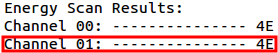
\includegraphics[height=25px]{Imagenes/Bitmap/Capitulo6/434sensingpre}}%
~
\subfloat[After start transmitting packets.]{\label{fig:cap6:434sensingpost}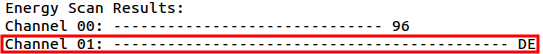
\includegraphics[height=25px]{Imagenes/Bitmap/Capitulo6/434sensingpost}}%

\caption{Spectrum sensgin at 434 MHz.}
\label{fig:cap6:434sensing}
\end{figure}


First scenario is conducted over 868 MHz band. This band posses 7 available channels when using a bitrate of 119,2 kbps. Transmitting device is making use of channel 4. Figure \ref{fig:cap6:868sensing} shows the energy scan traces deployed by the firmware.


\begin{figure}[!h]
\centering
\subfloat[Before start transmitting packets.]{\label{fig:cap6:868sensingpre}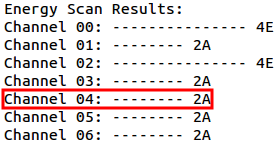
\includegraphics[height=70px]{Imagenes/Bitmap/Capitulo6/868sensingpre}}%
\qquad
\subfloat[After start transmitting packets.]{\label{fig:cap6:868sensingpost}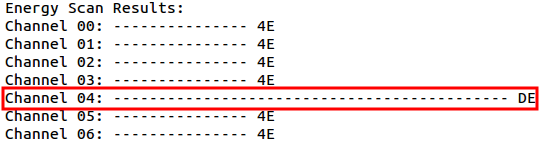
\includegraphics[height=70px]{Imagenes/Bitmap/Capitulo6/868sensingpost}}%

\caption{Spectrum sensgin at 868 MHz.}
\label{fig:cap6:868sensing}
\end{figure}

First scenario is conducted over 2.4 GHz band. This band posses 16 available channels. Transmitting device is making use of channel 4. Figure \ref{fig:cap6:2400sensing} shows the energy scan traces deployed by the firmware.

\begin{figure}[!h]
\centering
\subfloat[Before start transmitting packets.]{\label{fig:cap6:868sensingpre}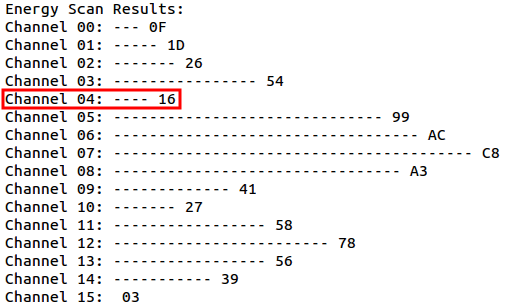
\includegraphics[height=130px]{Imagenes/Bitmap/Capitulo6/2400sensingpre}}%
~
\subfloat[After start transmitting packets.]{\label{fig:cap6:868sensingpost}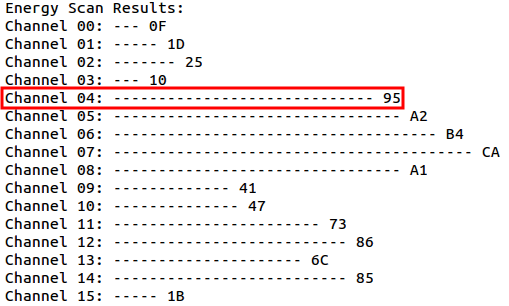
\includegraphics[height=130px]{Imagenes/Bitmap/Capitulo6/2400sensingpost}}%
\caption{Spectrum sensgin at 2.4 GHz.}
\label{fig:cap6:2400sensing}

\end{figure}

%-------------------------------------------------------------------
\section{Radio interfaces agility test}
%-------------------------------------------------------------------
\label{cap6:sec:radioagility}
%-------------------------------------------------------------------
This test evaluates how long changes over the \ac{RI}s take to be done. Parameters to change are \ac{TX} power, operation channel and energy modes. This test was fully available at the firmware. Table *********** ilustrates the results.



***************************************************

%-------------------------------------------------------------------
\section{Effective rate test}
%-------------------------------------------------------------------
\label{cap6:sec:radiocommunication}
%-------------------------------------------------------------------
Effective rate provided by the MRF49XA and MRF24J40 transceivers driven by the firmware was already described in \cite{juanpfc}. The obtained performance must match performance achieved at the \ac{CNGD}. That is why this checking supposes a partial test compared to the full previous characterization. However, it tries new unchecked aspects of the \ac{RI}s management and proves functionality. 

Most part of this test is obtained from the firmware, so the description is covered at its literature. Employed protocol at the test-bench, for simplicity, is MiWi$^{TM}$ P2P. The three \ac{RI}s are checked and different maintenance task periods for the protocol stack are tried. Main parameters set for the test follow:

\begin{itemize}
\item Payload
\item banksize
\item 255 Paquetes
\item VERIFY\_TRANSMIT 
\end{itemize}

Table ********** ilustrates the results for 434 MHz \ac{RI}.

************************************************************************

Conclusions

Table ********** ilustrates the results for 868 MHZ \ac{RI}.

***********************************

Conc.


Table ********** ilustrates the results for 2.4 GHz \ac{RI}.

***********************************

Conc.

%-------------------------------------------------------------------
\section{chargerSHIELD performance test}
%-------------------------------------------------------------------
\label{cap6:sec:charger}
%-------------------------------------------------------------------
As it was mantioned, small checkings were made during the mounting process. Nevertheless, this test shows the chargerSHIELD performance test facing a battery full charge operation.

%batteries
%charge
%c



% Variable local para emacs, para  que encuentre el fichero maestro de
% compilaci�n y funcionen mejor algunas teclas r�pidas de AucTeX
%%%
%%% Local Variables:
%%% mode: latex
%%% TeX-master: "../Tesis.tex"
%%% End:
